\documentclass{standalone}
\usepackage{graphicx}	
\usepackage{amssymb, amsmath}
\usepackage{color}

\usepackage{tikz}
\usetikzlibrary{intersections, backgrounds}
\usepackage{pgfmath}

\definecolor{light}{RGB}{220, 188, 188}
\definecolor{mid}{RGB}{185, 124, 124}
\definecolor{dark}{RGB}{143, 39, 39}
\definecolor{highlight}{RGB}{180, 31, 180}
\definecolor{gray10}{gray}{0.1}
\definecolor{gray20}{gray}{0.2}
\definecolor{gray30}{gray}{0.3}
\definecolor{gray40}{gray}{0.4}
\definecolor{gray60}{gray}{0.6}
\definecolor{gray70}{gray}{0.7}
\definecolor{gray80}{gray}{0.8}
\definecolor{gray90}{gray}{0.9}
\definecolor{gray95}{gray}{0.95}

\newcommand*{\offset}{0.025}

\begin{document}

\begin{tikzpicture}[scale=0.2, thick]

% Measurement 1
\pgfmathsetmacro{\dx}{0}

\fill[color=dark] (4 + \dx, 1.5) circle (1);
\filldraw[fill=white, draw=dark] (0 + \dx, 0) rectangle +(4, 3);

\draw[->, >=stealth, color=mid, line width=1] (-2 + \dx, 1.5) -- (0 + \dx, 1.5);
\node[right] at (-10.5 + \dx, 1.5) { $h_{n} = n\,\mathrm{m}$ };

\draw[-, color=mid, dashed, line width=1] (2 + \dx, 4) -- +(0, 5);

\fill[color=dark] (4 + \dx, 1.5 + 10) circle (1);
\filldraw[fill=white, draw=dark] (0 + \dx, 10) rectangle +(4, 3);

\draw[->, >=stealth, color=mid, line width=1] (-2 + \dx, 11.5) -- (0 + \dx, 11.5);
\node[right] at (-10.5 + \dx, 11.5) { $h_{2} = 2\,\mathrm{m}$ };

\fill[color=dark] (4 + \dx, 1.5 + 20) circle (1);
\filldraw[fill=white, draw=dark] (0 + \dx, 20) rectangle +(4, 3);

\draw[->, >=stealth, color=mid, line width=1] (-2 + \dx, 21.5) -- (0 + \dx, 21.5);
\node[right] at (-10.5 + \dx, 21.5) { $h_{1} = 1\,\mathrm{m}$ };

\fill[color=dark] (4 + \dx, 31.5) circle (1);
\filldraw[fill=white, draw=dark] (0 + \dx, 30) rectangle +(4, 3);

\draw[->, >=stealth, color=mid, line width=1] (-2 + \dx, 31.5) -- (0 + \dx, 31.5);
\node[right] at (-10.5 + \dx, 31.5) { $h_{0} = 0\,\mathrm{m}$ };

\node at (12.9 + \dx, 32.6) {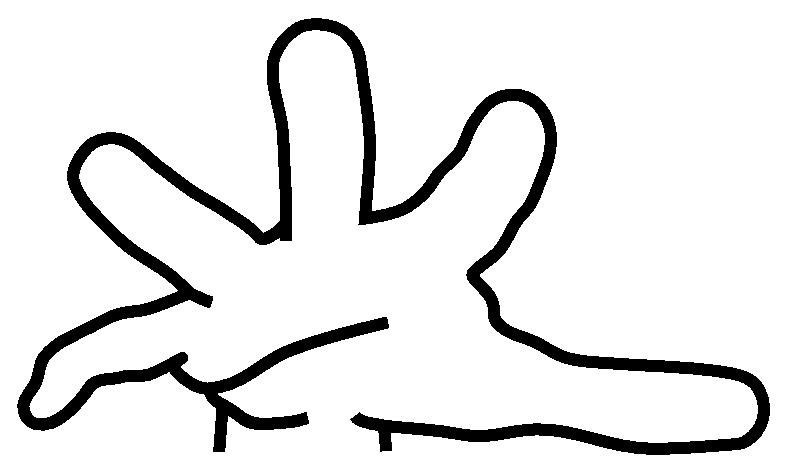
\includegraphics[width=1.4cm]{hands/open_hand.eps}};

\draw[->, >=stealth, color=mid, line width=1] (12.5 + \dx, 30) -- +(0, -6.5);

\fill[color=mid] (12.5 + \dx, 21.5) circle (2.1);

\draw[->, >=stealth, color=light, dashed, line width=1] (5.5 + \dx, 21.5) -- +(12.5, 0);
\node[right] at (18 + \dx, 21.5) { $\hat{t}_{\mathrm{fall}, 1} = t_{\mathrm{fall}}(h_{1}, g)$ };

% Measurement n
\pgfmathsetmacro{\dx}{50}

\fill[color=dark] (4 + \dx, 1.5) circle (1);
\filldraw[fill=white, draw=dark] (0 + \dx, 0) rectangle +(4, 3);

\draw[->, >=stealth, color=mid, line width=1] (-2 + \dx, 1.5) -- (0 + \dx, 1.5);
\node[right] at (-10.5 + \dx, 1.5) { $h_{n} = n\,\mathrm{m}$ };

\draw[-, color=mid, dashed, line width=1] (2 + \dx, 4) -- +(0, 5);

\fill[color=dark] (4 + \dx, 1.5 + 10) circle (1);
\filldraw[fill=white, draw=dark] (0 + \dx, 10) rectangle +(4, 3);

\draw[->, >=stealth, color=mid, line width=1] (-2 + \dx, 11.5) -- (0 + \dx, 11.5);
\node[right] at (-10.5 + \dx, 11.5) { $h_{2} = 2\,\mathrm{m}$ };

\fill[color=dark] (4 + \dx, 1.5 + 20) circle (1);
\filldraw[fill=white, draw=dark] (0 + \dx, 20) rectangle +(4, 3);

\draw[->, >=stealth, color=mid, line width=1] (-2 + \dx, 21.5) -- (0 + \dx, 21.5);
\node[right] at (-10.5 + \dx, 21.5) { $h_{1} = 1\,\mathrm{m}$ };

\fill[color=dark] (4 + \dx, 31.5) circle (1);
\filldraw[fill=white, draw=dark] (0 + \dx, 30) rectangle +(4, 3);

\draw[->, >=stealth, color=mid, line width=1] (-2 + \dx, 31.5) -- (0 + \dx, 31.5);
\node[right] at (-10.5 + \dx, 31.5) { $h_{0} = 0\,\mathrm{m}$ };

\node at (12.9 + \dx, 32.6) {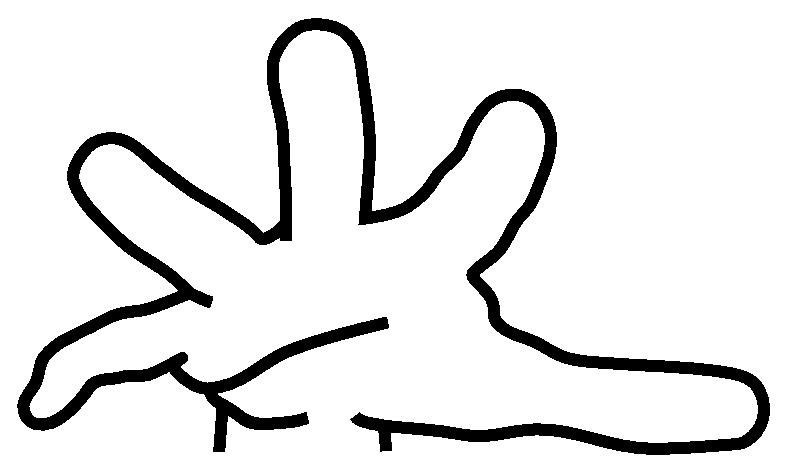
\includegraphics[width=1.4cm]{hands/open_hand.eps}};

\draw[-, >=stealth, color=mid, line width=1] (12.5 + \dx, 30) -- (12.5 + \dx, 9);
\draw[-, >=stealth, color=mid, dashed, line width=1] (12.5 + \dx, 9) -- (12.5 + \dx, 4);
\draw[->, >=stealth, color=mid, line width=1] (12.5 + \dx, 4) -- (12.5 + \dx, 3.5);

\fill[color=mid] (12.5 + \dx, 1.5) circle (2.1);

\draw[->, >=stealth, color=light, dashed, line width=1] (5.5 + \dx, 1.5) -- +(12.5, 0);
\node[right] at (18 + \dx, 1.5) { $\hat{t}_{\mathrm{fall}, n} = t_{\mathrm{fall}}(h_{n}, g)$ };

\end{tikzpicture}

\end{document}  